\documentclass{article}
\usepackage{iclr2027_conference,times}
% The four style files are byte-identical to the supplied v3 archive.
% Do not change the official geometry, line spacing, ruler or review header.
\usepackage[T1]{fontenc}
\usepackage[utf8]{inputenc}
\usepackage{amsmath,amssymb,mathtools}
\usepackage{graphicx,booktabs,array,tabularx,multirow}
\usepackage{xcolor}
\usepackage{algorithm,algpseudocode}
\usepackage{tikz}
\usetikzlibrary{arrows.meta,positioning,calc,fit}
\usepackage{microtype}
\usepackage[hidelinks]{hyperref}
\usepackage{url}
\newcommand{\method}{RePair}
\newcommand{\offoff}{Memory-OFF/Harness-OFF}
\newcommand{\ind}{\mathbf{1}}
\newcommand{\SR}{\operatorname{SR}}
\newcommand{\EVRY}{\operatorname{EVRY}}
\newcommand{\Benefit}{\mathsf{B}}
\newcommand{\Harm}{\mathsf{H}}
\newcommand{\NeutralS}{\mathsf{NS}}
\newcommand{\NeutralF}{\mathsf{NF}}
\newcommand{\Uncertain}{\mathsf{U}}
\newcommand{\pending}[1]{\textbf{[PENDING: #1]}}
\newcommand{\NA}{\textnormal{---}}
\newcolumntype{L}[1]{>{\raggedright\arraybackslash}p{#1}}
\makeatletter
\newcommand{\setresult}[2]{\expandafter\gdef\csname result@#1\endcsname{#2}}
\newcommand{\res}[1]{\ifcsname result@#1\endcsname\csname result@#1\endcsname\else\pending{#1}\fi}
\makeatother

\setresult{bench-unseen-strong-pick}{83.3}
\setresult{bench-unseen-strong-clean}{80.6}
\setresult{bench-unseen-strong-cool}{90.5}
\setresult{bench-unseen-strong-look}{83.3}
\setresult{bench-unseen-strong-heat}{78.3}
\setresult{bench-unseen-strong-pick2}{70.6}
\setresult{bench-unseen-strong-all}{81.3}
\setresult{bench-unseen-base-pick}{0.0}
\setresult{bench-unseen-base-clean}{0.0}
\setresult{bench-unseen-base-cool}{0.0}
\setresult{bench-unseen-base-look}{0.0}
\setresult{bench-unseen-base-heat}{4.3}
\setresult{bench-unseen-base-pick2}{0.0}
\setresult{bench-unseen-base-all}{0.7}
\setresult{bench-unseen-ours-pick}{\NA}
\setresult{bench-unseen-ours-clean}{\NA}
\setresult{bench-unseen-ours-cool}{\NA}
\setresult{bench-unseen-ours-look}{\NA}
\setresult{bench-unseen-ours-heat}{\NA}
\setresult{bench-unseen-ours-pick2}{\NA}
\setresult{bench-unseen-ours-all}{\NA}
\setresult{bench-unseen-skillrl-pick}{37.5}
\setresult{bench-unseen-skillrl-clean}{41.9}
\setresult{bench-unseen-skillrl-cool}{61.9}
\setresult{bench-unseen-skillrl-look}{44.4}
\setresult{bench-unseen-skillrl-heat}{43.5}
\setresult{bench-unseen-skillrl-pick2}{11.8}
\setresult{bench-unseen-skillrl-all}{41.0}
\setresult{bench-unseen-gigpo-pick}{87.5}
\setresult{bench-unseen-gigpo-clean}{87.1}
\setresult{bench-unseen-gigpo-cool}{95.2}
\setresult{bench-unseen-gigpo-look}{88.9}
\setresult{bench-unseen-gigpo-heat}{95.7}
\setresult{bench-unseen-gigpo-pick2}{94.1}
\setresult{bench-unseen-gigpo-all}{91.0}
\setresult{bench-unseen-seed-pick}{91.7}
\setresult{bench-unseen-seed-clean}{83.9}
\setresult{bench-unseen-seed-cool}{71.4}
\setresult{bench-unseen-seed-look}{11.1}
\setresult{bench-unseen-seed-heat}{95.7}
\setresult{bench-unseen-seed-pick2}{35.3}
\setresult{bench-unseen-seed-all}{69.4}
\setresult{bench-unseen-agentg2-pick}{79.2}
\setresult{bench-unseen-agentg2-clean}{87.1}
\setresult{bench-unseen-agentg2-cool}{85.7}
\setresult{bench-unseen-agentg2-look}{50.0}
\setresult{bench-unseen-agentg2-heat}{78.3}
\setresult{bench-unseen-agentg2-pick2}{94.1}
\setresult{bench-unseen-agentg2-all}{79.9}
\setresult{bench-unseen-opid-pick}{54.2}
\setresult{bench-unseen-opid-clean}{22.6}
\setresult{bench-unseen-opid-cool}{19.0}
\setresult{bench-unseen-opid-look}{11.1}
\setresult{bench-unseen-opid-heat}{52.2}
\setresult{bench-unseen-opid-pick2}{5.9}
\setresult{bench-unseen-opid-all}{29.1}
\setresult{bench-seen-strong-pick}{88.6}
\setresult{bench-seen-strong-clean}{59.3}
\setresult{bench-seen-strong-cool}{72.0}
\setresult{bench-seen-strong-look}{84.6}
\setresult{bench-seen-strong-heat}{93.8}
\setresult{bench-seen-strong-pick2}{58.3}
\setresult{bench-seen-strong-all}{75.0}
\setresult{bench-seen-base-pick}{0.0}
\setresult{bench-seen-base-clean}{0.0}
\setresult{bench-seen-base-cool}{0.0}
\setresult{bench-seen-base-look}{0.0}
\setresult{bench-seen-base-heat}{0.0}
\setresult{bench-seen-base-pick2}{4.2}
\setresult{bench-seen-base-all}{0.7}
\setresult{bench-seen-ours-pick}{\NA}
\setresult{bench-seen-ours-clean}{\NA}
\setresult{bench-seen-ours-cool}{\NA}
\setresult{bench-seen-ours-look}{\NA}
\setresult{bench-seen-ours-heat}{\NA}
\setresult{bench-seen-ours-pick2}{\NA}
\setresult{bench-seen-ours-all}{\NA}
\setresult{bench-seen-skillrl-pick}{60.0}
\setresult{bench-seen-skillrl-clean}{51.9}
\setresult{bench-seen-skillrl-cool}{68.0}
\setresult{bench-seen-skillrl-look}{46.2}
\setresult{bench-seen-skillrl-heat}{50.0}
\setresult{bench-seen-skillrl-pick2}{20.8}
\setresult{bench-seen-skillrl-all}{50.7}
\setresult{bench-seen-gigpo-pick}{100.0}
\setresult{bench-seen-gigpo-clean}{96.3}
\setresult{bench-seen-gigpo-cool}{88.0}
\setresult{bench-seen-gigpo-look}{92.3}
\setresult{bench-seen-gigpo-heat}{100.0}
\setresult{bench-seen-gigpo-pick2}{95.8}
\setresult{bench-seen-gigpo-all}{95.7}
\setresult{bench-seen-seed-pick}{100.0}
\setresult{bench-seen-seed-clean}{100.0}
\setresult{bench-seen-seed-cool}{64.0}
\setresult{bench-seen-seed-look}{46.2}
\setresult{bench-seen-seed-heat}{81.2}
\setresult{bench-seen-seed-pick2}{54.2}
\setresult{bench-seen-seed-all}{78.6}
\setresult{bench-seen-agentg2-pick}{97.1}
\setresult{bench-seen-agentg2-clean}{96.3}
\setresult{bench-seen-agentg2-cool}{84.0}
\setresult{bench-seen-agentg2-look}{76.9}
\setresult{bench-seen-agentg2-heat}{62.5}
\setresult{bench-seen-agentg2-pick2}{91.7}
\setresult{bench-seen-agentg2-all}{87.9}
\setresult{bench-seen-opid-pick}{42.9}
\setresult{bench-seen-opid-clean}{51.9}
\setresult{bench-seen-opid-cool}{20.0}
\setresult{bench-seen-opid-look}{15.4}
\setresult{bench-seen-opid-heat}{43.8}
\setresult{bench-seen-opid-pick2}{29.2}
\setresult{bench-seen-opid-all}{35.7}

\title{From Plausible Repairs to Policy Capability}
\author{Anonymous authors}
\hypersetup{pdftitle={From Plausible Repairs to Policy Capability},pdfauthor={Anonymous authors}}
% Anonymous submission mode. Do not enable \iclrfinalcopy.
\begin{document}
\maketitle
\begin{abstract}
A language model can propose a plausible correction for a failed attempt without knowing whether it will help the agent finish. Even when an intervention works, deciding what the policy should learn from it is a separate problem. We introduce \method{}, a research harness that connects failure analysis to policy learning through same-state, paired environment tests. Only interventions that repeatedly improve terminal completion become positive training evidence. A dual-view representation pairs a deployable action with training-only supervision for subgoals, expected progress, and recovery; evaluation then removes external memory and intervention. An ALFWorld study with Qwen2.5-3B-Instruct exposes a gap between these stages. Five development rounds produce one stable beneficial intervention among 21 source-state experiments. A subsequent executable-strategy validation finds four among five selected states, but these successes are completed by the intervention programs themselves. Training on their eight dual-view examples leaves scaffold-free selection success unchanged at 3 of 355 tasks, with one gain and one regression. The result separates useful intervention from acquired capability: environment verification can establish what works at a state without establishing that a small policy has learned to reproduce it. \method{} makes that distinction observable and identifies incomplete action coverage and persistent execution errors as concrete targets for further study.
\end{abstract}

\section{Introduction}
\label{sec:introduction}
A failed attempt tells a language agent that something went wrong. It does
not tell the agent what to learn. In a long task, failure may follow an
unproductive search, a missed change of subgoal, or an earlier error from
which the agent never recovered. A research model can inspect the
trajectory and suggest a correction. Reflection-based self-training uses
such feedback to improve generated samples \citep{dou2024rerest}.
Yet a convincing suggestion is still a hypothesis
about the policy's future behavior. Opening a cabinet instead of continuing
to search might reveal the needed object, or it might spend the remaining
budget and leave the task unsolved. The useful question is therefore concrete:
what happens when \emph{this policy} takes the proposed change from
\emph{that state}?

This question sits at a critical handoff in agent self-improvement. Memory
and harness adaptation can preserve experience outside the model
\citep{shinn2023reflexion,yu2026recuris}; policy training can carry useful
experience into the model parameters themselves
\citep{chen2026evotrainer,yang2026frontis}. The object we ultimately want to
retain is a policy that performs better when these external aids are
removed. A stronger intervention can improve the assisted trajectory
while leaving that object unchanged. Aspire shows why completing the
update loop is insufficient: agents can execute training while hidden-evaluation
gains remain sparse or unstable \citep{wu2026aspire}. We study the smaller,
more testable step between these two ends---how evidence from a failed attempt
becomes supervision that still helps after the research process is gone.

Prior work already supplies important pieces. CSO tests alternative actions
through policy continuation and learns from verified preferences
\citep{li2026cso}. SIRI validates skill-guided rollouts and distills useful
actions into an unassisted policy \citep{he2026siri}. OPID and SEED turn
trajectory hindsight into skills whose effect on action probabilities guides
policy learning \citep{yang2026opid,wu2026seed}. These advances make two
questions especially salient. First, which failure-derived changes actually
deserve to enter training? Second, once a change has earned that evidence,
what information should the learner receive from it?

The first question requires a baseline for the counterfactual. Restarting a
failed attempt gives the policy another opportunity to succeed even without
the proposed change. RePair therefore restores the source decision state and
runs two matched continuations: the registered baseline action and the
candidate intervention, with the same frozen policy available for subsequent
decisions. A bounded intervention can itself complete the task; its success
then measures the intervention's utility, not autonomous policy behavior.
The terminal outcomes measure whether adding the intervention changes
completion from that point. This same-state comparison
turns a plausible correction into experimentally grounded evidence.

The second question begins after verification. An action target teaches the
learner what to do at the source state. A compact strategy target can also
teach the active subgoal, the progress signal to watch for, and the condition
for changing course. In the cabinet example, opening the door is one action;
recognizing what observation would complete the search, and how to recover if
the object is absent, describes the decision structure around that action.
The two targets define a controlled comparison on the same verified states
and corrected actions. Here we instantiate the dual-view update and evaluate
its descendant through the original action-only interface, with external
failure memory and repair intervention disabled. An action-only training
control remains necessary to isolate the auxiliary view's contribution.

We introduce \method{} to make this handoff measurable end to end
(Figure~\ref{fig:framework}). Failure analysis and cross-round experience
help propose testable changes; same-state continuations determine which ones
become positive evidence; action and strategy targets specify
what enters learning; scaffold-free evaluation measures what remains in the
policy. The surrounding Analyzer, Planner, and
memory machinery supports this sequence, while the empirical study tracks
which of these handoffs actually succeeds.

Our ALFWorld study starts from Qwen2.5-3B-Instruct. Across five development
rounds, most verified interventions leave both branches unsuccessful.
Trace analysis locates a recurring failure: a local correction executes,
but the continuation policy misses the next prerequisite or repeats an
already completed action. A later validation makes more of the proposed
strategy executable and obtains stable terminal benefits. Yet training on
four such sources does not improve full-task selection success. These
observations locate the unresolved handoff: a program can finish a task
while the training examples teach only its initial decision. We report
the trace and supervision evidence behind this gap and measure its
consequence for the policy after external assistance is removed.

\section{RePair}
\label{sec:method}
\begin{figure}[t]
\centering
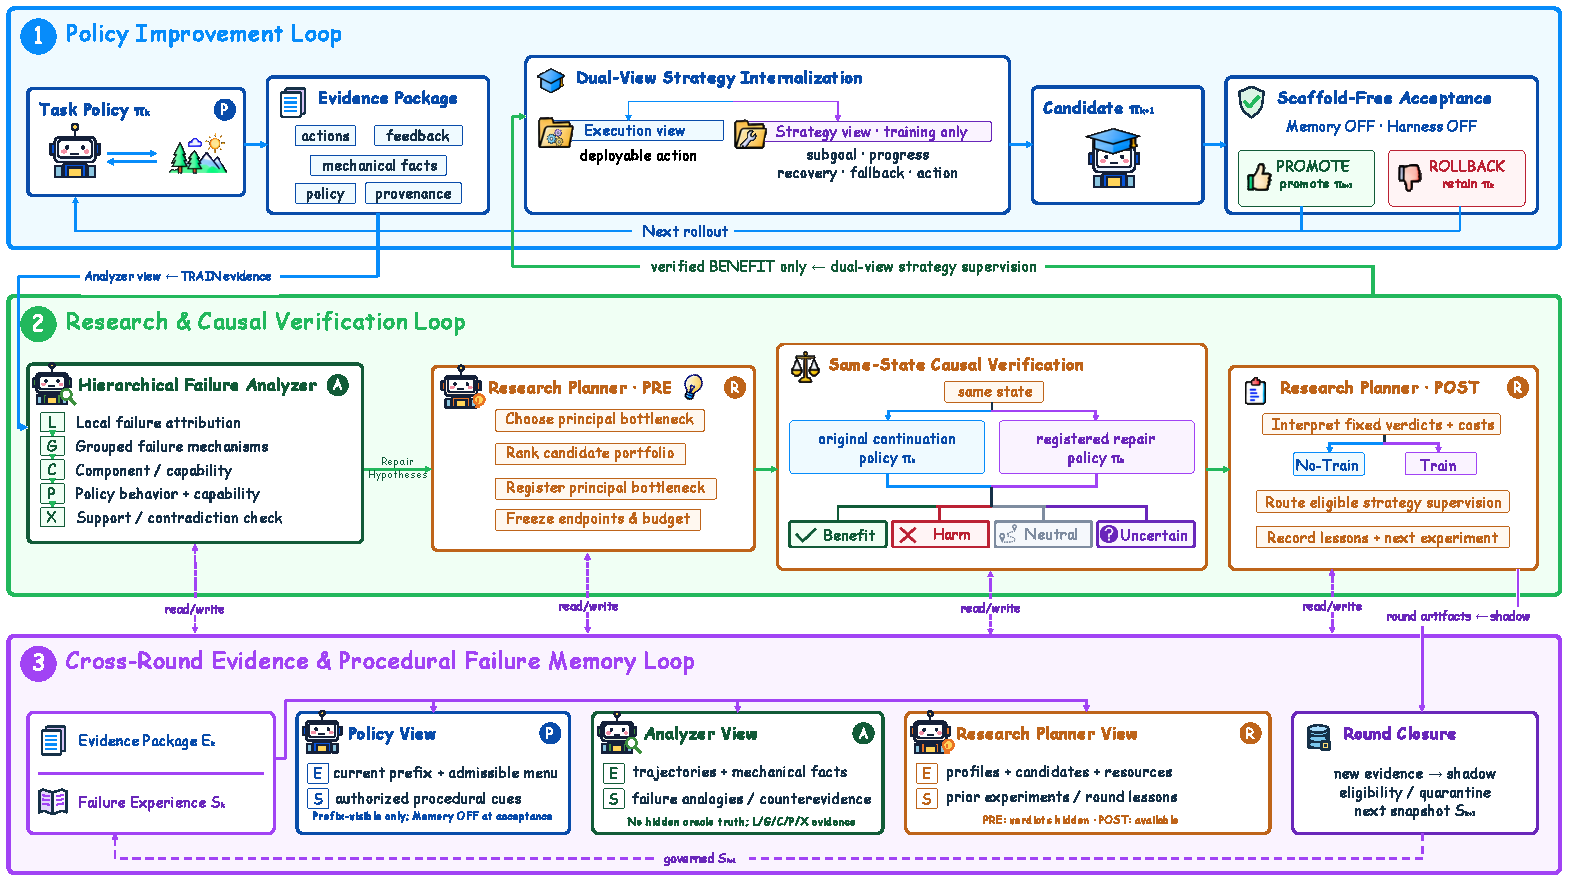
\includegraphics[width=\linewidth]{figures/repair_overview_cropped.pdf}
\caption{\textbf{RePair in context.} The paper follows the scientific path from failure-derived hypotheses through same-state verification, policy supervision, and scaffold-free acceptance. The research and memory loops support proposal selection and carry completed evidence across rounds; Section~\ref{sec:internalization} defines action-only and dual-view targets from verified evidence.}
\label{fig:framework}
\end{figure}

\method{} treats a repair as an experiment before treating it as supervision.
We follow that repair from its source state through testing, training, and
evaluation. Figure~\ref{fig:framework} shows the surrounding research loop;
Appendix~\ref{app:research} describes its analysis and memory mechanisms.

\subsection{Starting from a Failed Attempt}
\label{sec:setup-formal}
Let $\pi_k$ be the task policy entering round $k$. Its input contains a goal,
current observation, recent executed actions and feedback, and an admissible
action menu. We collect trajectories on the training split and retain their
actions, observations, budgets, and terminal outcomes. Completed task failures
supply the repair candidates; infrastructure incidents have their own
execution records.

Each candidate is tied to a recoverable decision state $x$ and the context
$c(x)$ visible to the policy. The source record fixes the checkpoint,
baseline action, action menu, and remaining budget. Environment-restoration
information stays outside $c(x)$. This distinction lets us restore the
experiment while preserving the information available to the agent.

A useful source state precedes a decision the proposal can change. For
example, continuing to search after the target has been found and searching
before it has been found can require different corrections, even if both
trajectories eventually fail. The source context anchors the proposal to
which subgoal is still active and what the agent has already observed.
This makes the unit of investigation a decision within a task.

\subsection{Proposing a Repair That Can Be Tested}
\label{sec:proposal}
The research models inspect a failed trajectory, connect local errors with
recurring failure patterns, and consult earlier repairs and counterexamples.
A planner chooses a principal bottleneck and a small portfolio of tests.
Each proposal specifies a source state, an executable repair $r$, and a
compact strategy describing its subgoal, expected progress, and recovery
conditions. The intervention is an action or a bounded program with conditions
grounded in visible observations and explicit termination rules. Earlier rounds use one action or an
option of at most four actions; the later validation uses ordered guarded
phases within the same remaining environment budget. Its payload, strategy description,
endpoint, and budget are fixed before the environment test.

The researcher receives trajectory observations and mechanical execution
facts, including admissible actions and feedback. It can reason about
search, subgoal transitions, prerequisites, or recovery, but the proposal
must identify how to test that reasoning in the environment. Hidden
restoration state remains with the verifier. This division lets the
research model suggest a high-level strategy while the environment
determines whether its executable realization helps.

This makes the proposal concrete. A suggestion to ``search more carefully''
becomes a particular action or option at a particular state. Related failures
help the researcher distinguish an isolated invalid action from a recurring
problem, such as continuing an exhausted search. Historical experience
supplies possible next steps and the conditions under which they previously
helped. These sources guide where to spend the test budget; current paired
rollouts measure the effect on $\pi_k$.

Research within a round reads a fixed history snapshot. The proposal can
use a lesson from an earlier round, but its action and strategy are settled
before the current outcomes are revealed. Completed outcomes then become
historical evidence for the next round (Appendix~\ref{app:views}). This
allows research to accumulate experience while keeping each proposed
intervention tied to a specific test.

\subsection{Returning to the Same State}
\label{sec:verification}
For a candidate $(x,r)$, we restore $x$ twice. Branch $F_0$ executes the
registered baseline action $a_0$; branch $F_1$ executes the repair. If the task remains unfinished, the same frozen policy $\pi_k$ supplies
subsequent decisions:
\begin{equation}
\begin{aligned}
F_0 &: x\xrightarrow{a_0}x'_0\xrightarrow{\pi_k}Y^{(0)},\\
F_1 &: x\xrightarrow{r}x'_1\xrightarrow{\pi_k}Y^{(1)}.
\end{aligned}
\label{eq:branches}
\end{equation}
Here $Y^{(b)}\in\{0,1\}$ is terminal task success. We repeat the paired
comparison five times. Each pair shares the starting state and visible
context, checkpoint, base prompt interface, memory snapshot, remaining budget, and
paired seed protocol. In the later strategy validation, $r$ also includes
a registered strategy cue on F1 continuation calls; the treatment is the
program and cue together, not an isolated action change. The baseline is a fresh policy continuation and can succeed
even though the source episode failed.

After the intervention the branches are free to diverge; that divergence
is precisely what the repair is meant to cause. Every intervention action
consumes the remaining interaction budget. For an option, the test covers
the complete registered option, with admissibility checked at each reached
state. Across repetitions, the joint $F_0/F_1$ outcomes describe the local,
policy-conditioned effect of the proposed change. Appendix~\ref{app:restoration}
gives the restoration and execution checks.

Keeping the continuation policy fixed is central to this test. Replacing it
with a stronger teacher asks whether the teacher can finish after the
intervention. When continuation is needed, using $\pi_k$ tests whether the learner can
use the state reached by the intervention. If the program already reaches
success, no policy continuation is required; we explicitly count this case. In the cabinet
example, exposing an object is useful only to the extent that the remaining
policy can turn that opportunity into task completion within the budget.
Intermediate progress helps explain the branches; terminal success supplies
the effect label.

\subsection{Selecting Repairs for Learning}
\label{sec:eligibility}
An independent verifier reads the paired outcomes. A candidate receives
\emph{Benefit} when at least four of the five valid pairs change failure to
success and none changes success to failure. The symmetric rule gives
\emph{Harm}. Stable success in both branches and stable failure in both
branches give two neutral outcomes; other complete results are uncertain.
We use these repetitions to assess stability at the selected state;
Appendix~\ref{app:labels} gives the exact counts and treatment of incomplete tests.

Let $\mathcal I_k$ contain completed interventions whose source and training
records agree with the executed test. Positive supervision is the Benefit subset:
\begin{equation}
\mathcal D_k^+=\{i\in\mathcal I_k:L_i=\Benefit\}.
\label{eq:eligibility}
\end{equation}
A change that repeatedly helps the current policy thus becomes a candidate
lesson. The verifier selects on its executed effect; the associated strategy
remains the description fixed before testing.

The remaining outcomes also inform research. Repeated success in both
branches suggests that this correction is unnecessary under the tested
conditions. Repeated failure leaves an unresolved difficulty, and a harmful
intervention supplies a counterexample to the proposal. The planner uses
these outcomes and their costs to choose TRAIN or NO-TRAIN and to guide
later tests. This gives negative experiments a role without putting them
in the positive-supervision set.

\subsection{Learning an Action or Learning Its Strategy}
\label{sec:internalization}
A verified intervention tells us which decision helped. We now ask how to
teach it. A historical data-path audit made this question concrete: an
action-only materialization retained the chosen actions as targets while
richer strategy information remained upstream
(Appendix~\ref{app:historical}). We therefore make that information an explicit auxiliary prediction
target. The action-only formulation below defines the corresponding
control; the completed update in this study uses dual views.

\emph{Action-only} supervision uses the deployment context $c_i$ and the
target $a_i$, serialized as \texttt{\{"action":"..."\}}. Let $c_i^s$
denote the same legal source context with a fixed training-only instruction.
\emph{Dual-view} supervision keeps the action examples and adds a strategy view:
\begin{equation}
\begin{aligned}
\mathcal T_{\mathrm{action}}&=\{(c_i,a_i):i\in\mathcal D_k^+\},\\
\mathcal T_{\mathrm{dual}}&=\mathcal T_{\mathrm{action}}\cup
\{(c_i^s,s_i):i\in\mathcal D_k^+\}.
\end{aligned}
\label{eq:training-views}
\end{equation}
The strategy instruction requests a compact response $s_i$ with
the bottleneck, subgoal, expected event and state change, progress criterion,
recovery trigger, fallback condition, and action. These fields relate a
choice to the task: the subgoal says what it is meant to accomplish, the
progress criterion says what to check next, and recovery conditions say
when to change course. Table~\ref{tab:views-example} illustrates the
information added to an action target.
\begin{table}[H]
\caption{\textbf{What each training view teaches.} Schematic example:
the agent is looking for an object beside a closed cabinet, and
\texttt{open cabinet 1} is admissible. The auxiliary view adds prospective
task information to the same action. This illustrates target content.}
\label{tab:views-example}
\centering\small
\begin{tabularx}{\linewidth}{@{}L{1.10in}X@{}}
\toprule
View & Supervised content\\
\midrule
Execution & \texttt{\{"action":"open cabinet 1"\}}\\
Strategy & Subgoal: inspect the cabinet. Expected progress: its contents
become visible. Check: whether the target is present. Recovery/fallback:
if it is absent, continue the search elsewhere. Action:
\texttt{open cabinet 1}.\\
\bottomrule
\end{tabularx}
\end{table}


The response uses the strategy registered before verification. Expected
progress is prospective: it states what to look for in subsequent feedback.
Realized future outcomes, rewards, and effect labels are excluded from
prediction targets. In the completed update, each source contributes its initial action and
one strategy response. The later actions of a successful intervention are
not expanded into additional execution-view examples. This distinction
between verified program coverage and supervised action coverage matters
for interpreting transfer.

The two views update the same policy weights through supervised
assistant-token loss. Prompt tokens are masked; the auxiliary response
makes the strategy itself a prediction target. The native-label check
confirms that both action and substantive strategy tokens contribute to
that loss. The fixed auxiliary instruction gives this training task its
own output format while the original parser continues to accept exactly
one action field. Evaluation uses the execution view directly, with no
strategy-generation step or additional research-model call.

A controlled representation comparison would start both conditions from
the same parent and evidence, and include an equal-compute action-only
control. Those controls are not completed here. We report the executed
dual-view labels, tokens, and optimizer steps in
Appendix~\ref{app:training-details}; the observed parent--candidate change
therefore measures this update as a whole.

\subsection{Removing the Assistance}
\label{sec:iteration}
The final test belongs to the policy. We remove external failure memory and
repair takeover and compare candidate $\pi'$ with parent $\pi$ under the
original action interface. For task $t$ and seed $j$, let $Y_{tj}(\pi)$ denote
terminal success in this scaffold-free setting. We measure
\begin{equation}
\begin{aligned}
\widehat{\SR}_{\mathcal D}(\pi)
&=\frac{1}{|\mathcal D|}\sum_{t\in\mathcal D}
\frac{1}{J_{\mathrm{eval}}}\sum_{j=1}^{J_{\mathrm{eval}}}Y_{tj}(\pi),\\
\Delta^{\mathcal D}_{\mathrm{policy}}(\pi',\pi)
&=\widehat{\SR}_{\mathcal D}(\pi')-\widehat{\SR}_{\mathcal D}(\pi).
\end{aligned}
\label{eq:policy-eval}
\end{equation}
The goal, observations, ordinary within-task history, admissible menu, and
strict action parser remain available to both policies. Evaluation starts
at each task's initial state, so the learned model also has to reach useful
decisions without being placed at a selected failure point. This extends
the local intervention test to complete task behavior.

During the improvement loop, an independent predeclared acceptance rule
compares candidate and parent on training-side selection tasks, after
integrity checks. In the final validation, success count is primary; ties
use the mean terminal fraction of satisfied goal conditions, evaluated
outside the policy input. No clear improvement retains the parent. A NO-TRAIN decision retains the
parent. The retained policy collects fresh failures for the next round, and
completed research updates the next history snapshot. The final seen and
unseen benchmark sets are evaluated after selection; their scores stay
outside this adaptive loop. Appendix~\ref{app:research} specifies the full
return from one round to the next.

\section{Experimental Study}
\label{sec:experimental-setup}
We examine the path from a tested correction to an unassisted policy in a
development campaign and a subsequent one-update validation. The campaign
and validation are sequential diagnostics with implementation changes,
not randomized comparisons of repair representations.

\subsection{Setting and Comparisons}
\label{sec:experiment-design}
\paragraph{Tasks and policy.}
We use text-based ALFWorld \citep{shridhar2021alfworld} and the
Qwen2.5-3B-Instruct lineage \citep{qwen2025report}, updated with LoRA
\citep{hu2021lora}. The 3,553 training games are partitioned into 2,843
TRAIN\_UPDATE, 355 TRAIN\_SELECT, and 355 TRAIN\_AUDIT games. Only the
first pool supplies repair and learning evidence. Selection uses the
second pool. The final benchmark has 134 unseen and 140 seen games,
kept outside adaptive research and checkpoint selection.

\paragraph{Execution and statistical units.}
The policy receives the goal, current observation, eight executed
transitions, interface feedback, and the complete admissible menu. The
strict interface accepts one JSON action. Episodes allow 30 environment
steps and 60 policy attempts, with termination after three consecutive
nonexecuted attempts. Repair verification uses five paired seeds
(17, 31, 47, 73, 101); the final selection comparison uses one paired seed
(17) on all 355 tasks. Repetitions at one source are not independent
tasks. We report exact counts and descriptive differences for one trained
candidate, without claims of significance or training-seed robustness.
Appendix~\ref{app:configuration} records the executed configuration.

\paragraph{Scope of the evidence.}
We report completed intervention tests, native training labels, and paired
selection outcomes. Matched action-only, equal-compute, filter, hierarchy,
and memory ablations have not been completed for this update. The released
checkpoint benchmark supplies external context; it does not isolate
RePair's components. The RePair candidate has no completed final
seen/unseen benchmark result.

\subsection{Which Repairs Help the Current Policy?}
\label{sec:verification-results}
\begin{table}[!htbp]
\caption{\textbf{Completed same-state tests.} Counts are source-state
experiments; each has five pairs and ten branches. N denotes stable
neutral failure. Validations reuse R5 evidence and change the selected
portfolio and executable representation. They are not matched ablations.}
\label{tab:verification}\centering\small
\begin{tabular}{lrrrrr}\toprule
Run & States & Benefit & Harm & N & Uncertain\\\midrule
R1 & 11 & 0 & 0 & 11 & 0\\
R2 & 6 & 1 & 0 & 5 & 0\\
R3 & 2 & 0 & 0 & 2 & 0\\
R4 & 1 & 0 & 0 & 1 & 0\\
R5 & 1 & 0 & 0 & 1 & 0\\\midrule
Guarded-strategy validation & 17 & 0 & 0 & 16 & 1\\
Executable-strategy validation & 5 & 4 & 0 & 1 & 0\\\bottomrule
\end{tabular}
\end{table}

Table~\ref{tab:verification} separates the five development rounds from two
later validations that reuse R5 trajectories and Analyzer outputs. The
development rounds yield one stable Benefit among 21 tested states;
the other 20 are neutral failures. The first guarded-strategy validation
has no stable Benefit among 17 states, although two of its 85 pairs show
an F1-only success at the same source. The later executable-strategy
validation yields four stable Benefits among five selected states.
All five repetitions succeed in F1 and fail in F0 at each beneficial
state. The higher yield motivates examining what the successful programs do;
the sequentially selected portfolios leave the effect of each design change unresolved.

The trajectories explain why many valid corrections remain neutral.
In R3, reaching the fridge enables cooling an egg, but the continuation
then cools it 25 times instead of placing it. In a CD task, navigation
reveals the target, but the policy attempts placement three times without
first acquiring it. In R4, using a lamp is followed by 28 examinations of
the same side table. The intervention executes; the remaining dependency
chain fails. Appendix~\ref{app:behavior} records further cases.

The four beneficial programs in the later validation execute two, four,
six, and four actions, respectively, covering cleaning, placement,
heating-and-placement, and object-in-light tasks. All 20 successful F1
branches finish within the registered program, with zero subsequent
policy calls. The successful behavior therefore comes from the programs at these
selected states. Whether their verified actions become useful lessons
for the policy is the next question.

The heated-cup case makes the distinction concrete. From the restored
state, the program acquires the cup, reaches the microwave, heats it,
opens the microwave, reaches the cabinet, and places the cup. Completion
follows this six-action sequence without another policy decision. In
the remaining neutral case, the program locates and acquires a credit
card, but the three subsequent policy calls fail to execute and placement
remains unfinished. A useful intermediate state becomes a completed task
only when the remaining prerequisites are also resolved. These cases
locate the handoff that a trained policy would need to learn.

\subsection{What Enters Training?}
\label{sec:target-results}\label{sec:ablations}
The four Benefit states contribute four execution views and four strategy
views. The native-label audit counts 51 action-view and 2,546 strategy-view
loss-bearing tokens per pass. Four passes produce eight optimizer updates
and 10,388 supervised token exposures. Prompt and padding tokens are
masked. The current adapter teaches the initial action and associated strategy
at each source, leaving the remaining successful actions without
stepwise execution targets.
\begin{table}[!htbp]
\caption{\textbf{Verified program coverage and supervised action coverage.}
Each row is one Benefit source, with five successful F1 repetitions and
zero policy continuation calls. Action counts are per repetition; native
training counts are per source, not multiplied by the five seeds.}
\label{tab:coverage}\centering\small
\begin{tabularx}{\linewidth}{Xrrr}\toprule
Repair task & Program actions & Action targets & Strategy targets\\\midrule
Clean pan & 2 & 1 & 1\\
Place potato & 4 & 1 & 1\\
Heat and place cup & 6 & 1 & 1\\
Examine newspaper with lamp & 4 & 1 & 1\\\midrule
Total & 16 & 4 & 4\\\bottomrule
\end{tabularx}
\end{table}


For example, the heated-cup training pair supplies an action target for
acquiring the cup and a strategy description of the intended plan. The
five later action positions are exercised by the verifier but are not
separate action-prediction examples. The auxiliary view may communicate
the plan, while execution from the intervening observations remains a
generalization demand. Table~\ref{tab:coverage} makes this coverage gap
visible without treating each repetition as a new training source.

Thus verification coverage and training coverage differ: a program can
complete several prerequisites while the action target teaches only its
first decision. Strategy text supplies most supervised tokens; its gradient influence
also depends on token losses and accumulation-group composition
(Appendix~\ref{app:training-details}). The comparison below tests this
eight-example update as a whole. Isolating the strategy objective would
require an action-only update from the same four sources.

\subsection{What Remains After the Research Harness Is Removed?}
\label{sec:main-results}
\begin{table}[!htbp]
\caption{\textbf{Scaffold-free selection after the dual-view update.}
TRAIN\_SELECT only: 355 paired tasks, seed 17, one trained candidate.
Counts concern episodes except where marked as calls. Goal completion
is the mean terminal fraction of satisfied environment goal conditions.}
\label{tab:ablations}\centering
\begin{tabularx}{\linewidth}{Xrr}\toprule
Measure & Parent & Candidate\\\midrule
Task successes & 3 / 355 & 3 / 355\\
Mean goal-condition completion (\%) & 10.845 & 10.704\\
Consecutive-nonexecution terminations & 261 & 252\\
Environment-budget terminations & 91 & 100\\
Out-of-menu actions (calls) & 1,556 & 1,612\\
Format failures (calls) & 135 & 119\\\bottomrule
\end{tabularx}
\end{table}

On TRAIN\_SELECT, both parent and candidate solve 3 of 355 tasks (0.85\%).
Two successes are shared; one task improves and one regresses. Mean terminal
goal-condition completion decreases from 10.845\% to 10.704\%, so the
registered success-first, progress-on-ties rule retains the parent.
The comparison comprises 710 completed episodes with memory and
intervention disabled. It is a selection result, not a final benchmark.

Looking at task identities prevents the equal totals from hiding
redistribution: 351 tasks fail under both policies, two succeed under
both, and only two switch outcome. The secondary goal measure improves
on five tasks, worsens on six, and is unchanged on 344. We therefore find
neither a net completion gain nor a compensating aggregate progress gain
under this acceptance rule. The two discordant success outcomes support
an exact descriptive comparison, rather than a claim about training-seed
robustness.

Most failures concern execution rather than unavailable observations.
The parent and candidate terminate 261 and 252 tasks, respectively, after
consecutive nonexecuted attempts. Their traces contain 1,556 and 1,612
out-of-menu actions despite visible admissible menus. Fewer early stops
coexist with more budget-exhausted episodes (91 versus 100), leaving
terminal success unchanged. In a task requiring an alarm clock to be
examined with a desk lamp, both policies emit an unavailable examine
command even though the observation contains the clock and the menu
offers a take action. The missing step is therefore visible in the
interface; the policy fails to use it. This example links the aggregate
execution errors to a prerequisite failure of the same kind observed
after local repairs.

The existing reference-checkpoint benchmark is retained as task context
in Appendix~\ref{app:aggregation}; all policy-update conclusions here use
the paired TRAIN\_SELECT comparison.

\subsection{Research Cost and the Cross-Round Record}
\label{sec:discovery-results}
The five development rounds consume 210 completed verification branches
over 21 tested states. The guarded and executable-strategy validations
consume 170 and 50 branches, respectively. They reuse R5 collection and
analysis, so they are neither fresh formal rounds nor independent samples
of discovery yield. The last portfolio costs 50 branches for four Benefit
states, or 12.5 branches per Benefit, excluding upstream research and
earlier unsuccessful portfolios.

The campaign stops after five valid rounds under its three-round
no-promotion patience rule. One infrastructure-invalid attempt, repeated
engineering recoveries, and one user-authorized promotion exception remain
part of the record. The later validation completes training and selection
but encounters an ownership check during history closeout. We therefore
report its verified selection decision separately from campaign closure,
and make no claim of uninterrupted autonomous execution. Full API cost,
matched discovery efficiency, and further policy improvement remain
unmeasured in this study.

\section{Related Work}
\label{sec:related}
\paragraph{From failure to a tested correction.}
Reflexion uses linguistic feedback in later attempts
\citep{shinn2023reflexion}, and Re-ReST uses reflection and external feedback
to improve self-training data \citep{dou2024rerest}. AgentRx and TrajDebug
localize failures from execution evidence \citep{barke2026agentrx,qi2026trajdebug};
SAGE considers multiple failure hypotheses for research recovery
\citep{ma2026sage}. CSO goes from diagnosis to intervention, testing
alternative actions through policy continuation and learning verified
preferences \citep{li2026cso}. \method{} also tests corrections in the
environment, then traces which parts of the verified intervention enter training and
whether the resulting policy improves. This follows the correction beyond its local effect to the behavior
retained after training.

\paragraph{From guidance to policy learning.}
GiGPO addresses credit assignment in agent RL \citep{feng2025gigpo}, while
Agent-G$^2$ adapts the expert-prefix guidance used to start training rollouts
\citep{wang2026agentg2}. SkillRL develops a hierarchical skill library
\citep{xia2026skillrl}; SIRI tests skills and distills useful skill-guided
actions into an unassisted policy \citep{he2026siri}. OPID and SEED use the
probability shifts induced by hindsight skills as a dense learning signal
\citep{yang2026opid,wu2026seed}. Rationale supervision can also complement
ordinary task targets \citep{hsieh2023distilling}. Our formulation focuses on
state-bound failure repairs: the same tested actions supply either ordinary
action targets or those targets plus a training-only strategy view.
The distinction is in the supervision given to a shared learner while its
deployment interface stays fixed.

\paragraph{What carries across improvement rounds.}
Self-Harness and Recuris retain changes in external execution and memory
mechanisms \citep{zhang2026selfharness,yu2026recuris}. EvoTrainer couples
training-harness adaptation with policy learning \citep{chen2026evotrainer},
and Frontis-MA1 learns program-evolution operators from executable feedback
\citep{yang2026frontis}. HELIX organizes matched harness outcomes into
verified model-update records \citep{fan2026helix}. Aspire and PAST-Bench
examine whether updates and retained experience produce supported gains
\citep{wu2026aspire,xue2026past}. \method{} studies the passage into the task
policy: proposals are tested, their supervision is audited, and the updated
model is evaluated after the research assistance is removed. Its research
history can guide later experiments, while OFF/OFF evaluation measures
what each update leaves in the learner.

\section{Discussion and Limitations}
\label{sec:discussion}
The study locates two distinct obstacles. Early local corrections often
leave the policy facing an unresolved prerequisite or phase transition.
Making a larger part of the strategy executable can complete a task, but
that success may belong entirely to the intervention program. The later
dual-view update does not transfer this observed utility into higher
scaffold-free selection success.

The learner receives initial-action targets from just four source states,
whereas evaluation requires it to reach and complete these decisions from
task reset. This mismatch in both coverage and starting conditions offers
a plausible explanation for weak transfer. A controlled training comparison
is needed to establish its causal role. The trajectories
also reveal persistent menu and prerequisite errors. A useful next test
would match source states and training budget while varying coverage of
the verified continuation, before scaling the number of rounds. In particular, the current result
suggests measuring what the learner does after each verified intermediate
state, as well as from task reset. This would distinguish learning the
successful continuation from learning to reach its starting point.
Such a comparison follows directly from the observed gap; its outcome
remains an empirical question.

The revisions and portfolios were chosen sequentially, so their outcome
counts are descriptive. The 355-task comparison uses one seed and one
candidate; it measures neither training variability nor final benchmark
generalization. Matched action-only, filtering, equal-compute, and research-memory
comparisons, together with a final RePair benchmark evaluation, remain
open tests. The heterogeneous released baselines provide task context.
Our present evidence concerns the local-to-policy transfer gap in this
development study.

Five paired repetitions establish the registered stability criterion,
not statistical certainty, and failure-selected states provide limited
opportunities to measure harm. Human engineering recovery and a disclosed
promotion exception prevent interpreting the development campaign as
fully unattended. RePair's contribution here is the explicit separation
and measurement of these handoffs, including the observed absence of a retained policy gain.

\section{Conclusion}
\label{sec:conclusion}
RePair connects failure analysis, same-state verification, dual-view
supervision, and scaffold-free policy evaluation. Its ALFWorld study finds
that executable corrections can produce stable terminal benefits while
a small update from those corrections leaves independent task success
unchanged. The trace and supervision audits show where the handoff remains
incomplete: the intervention can perform a sequence that the action
training data does not teach in full. This establishes a concrete
experimental target for improving internalization, while keeping useful
research assistance distinct from capability retained by the policy.

\label{maintextend}
% Keep post-main sections on their own pages. Flush floats at each boundary.
\clearpage
\phantomsection
\pdfbookmark[0]{Statements}{statements}
\label{statementsstart}
\section*{AI Use Statement}
Generative AI was used in the research method and in its development.
External GPT API models supplied failure analyses, repair proposals,
PRE/POST planning, and strategy supervision; the recorded provider model
for the recent validation is \texttt{gpt-5.6-sol}. Qwen2.5-3B-Instruct and
its trained descendants generated task actions. ChatGPT and Codex assisted
with conceptual and experimental design, implementation and debugging,
data extraction and analysis, literature search, mathematical exposition,
English revision, figures, and LaTeX production. Task outcomes and effect
labels were computed from environment execution rather than accepted from
model judgments. Checks included source/result identity checks, tests,
native training-label audits, paired episode recounts, and document
compilation and layout inspection. The authors remain responsible for
the final claims, interpretation, and artifacts.

\section*{Ethics Statement}
The study concerns simulated household tasks and provides no evidence for
safe physical deployment. External research models process simulated
trajectory evidence. The accompanying numerical supplement excludes
credentials, private server locations, and identifying operational logs.
Third-party environments and checkpoints retain their original licenses
and access conditions. Regressions, unsuccessful tests, implementation
changes, and human intervention are disclosed to avoid conflating system
execution with autonomous capability improvement.

\section*{Reproducibility Statement}
Section~\ref{sec:method} defines the procedure;
Appendix~\ref{app:protocol} specifies interventions and training;
Appendix~\ref{app:experimental} gives the evaluation protocol and
checkpoint context; and Appendix~\ref{app:research} documents the campaign.
The accompanying anonymous numerical supplement contains the 355 paired
selection records, 50 validation branch summaries, training configuration,
and a script that recomputes the reported counts. It supports direct numerical
verification of the tables. Independently rerunning the GPU/API campaign
would additionally require model weights, environment replay assets, and
API access, which are outside this numerical supplement.

\clearpage
\phantomsection
\pdfbookmark[0]{References}{references}
\label{referencesstart}
\bibliography{references}
\bibliographystyle{iclr2027_conference}
\clearpage
\appendix
\phantomsection
\pdfbookmark[0]{Appendix}{appendix}
\section*{Appendix}
\label{appendixstart}
\section{Repair Tests and Training Details}
\label{app:protocol}
This appendix specifies the state restoration, evidence handling, and learning
procedure used in Section~\ref{sec:method}.

\subsection{Notation and Information Available to Each Role}
\label{app:views}
\begin{table}[htbp]
\caption{Notation for a repair, an improvement round, and an evaluation task.}
\centering
\begin{tabularx}{\linewidth}{lX}
\toprule
Symbol & Meaning\\\midrule
$\pi_k$ & Retained task policy entering round $k$.\\
$\widetilde\pi_{k+1}$ & Trained candidate awaiting the selection test.\\
$x,\ c(x)$ & Recoverable environment state and policy-visible context.\\
$r,\ a_0$ & Registered repair and current-policy baseline action.\\
$E_k,\ S_k$ & Current trajectory evidence and round-start experience snapshot.\\
$\mathcal U$ & Common predeclared set of failure units.\\
$\mathcal I_k$ & Completed interventions whose source and training records match the executed test.\\
$J_{\mathrm{eval}}$ & Repetitions per evaluation task; one in the primary benchmark.\\
$\mathcal D_k^+$ & Benefit subset used for positive supervision.\\
$A_k$ & Scaffold-free acceptance result for candidate policy $k+1$.\\
\bottomrule
\end{tabularx}
\end{table}

\begin{table}[htbp]
\caption{Research inputs and responsibilities. Current experiment outcomes
enter POST directly; historical retrieval reads the round-start snapshot.}
\centering
\begin{tabularx}{\linewidth}{L{0.82in}>{\raggedright\arraybackslash}X>{\raggedright\arraybackslash}X}
\toprule
Role & Available evidence & Responsibility\\\midrule
Task policy & Goal, visible prefix, menu; permitted procedural cues when memory is enabled & Select the next action. OFF/OFF evaluation removes the extra cues.\\
Analyzer & Trajectories, mechanical facts, failure analogies, counterexamples & Propose source-grounded failure hypotheses and repairs.\\
Planner PRE & Failure profiles, candidates, resources, earlier experiments & Select and register the intervention portfolio before current verdicts.\\
Planner POST & Registered PRE, fixed current verdicts and costs, earlier lessons & Interpret experiments and recommend TRAIN or NO-TRAIN.\\
Verifier & Executed paired traces and the fixed effect rule & Assign Benefit, Harm, neutral, or uncertain labels.\\
Acceptance rule & Candidate and parent results on training-side selection tasks & Apply the predeclared promotion and regression criteria.\\
\bottomrule
\end{tabularx}
\end{table}

A historical record retains starting conditions, the action/feedback sequence,
observed state changes, a wrong branch and its consequence, the repair,
applicability conditions, counterexamples, and effect provenance. Retrieval
identifies whether a record is an exact past observation or an analogy. Its
usefulness for the current policy is determined by a new experiment.
Within round $k$, historical reads use the immutable snapshot $S_k$.
New records accumulate in a shadow writeback store and become available as
history through $S_{k+1}$ after round closure. POST receives current verdicts
through its explicit experiment-result input. Hidden restoration state and
future outcomes are excluded from task-policy inputs.

\subsection{Restoring the Source and Executing the Repair}
\label{app:restoration}
The source record identifies the task/gamefile, source prefix and state,
policy checkpoint, prompt, initial menu, memory snapshot, candidate payload,
and remaining budget. Restoration uses an environment-supported snapshot
or a checked replay of the recorded prefix. The experiment records the
backend, replay checks, paired seed protocol, and restored-context equality;
the current validation uses checked public-prefix replay. Its five
continuation seed slots are 17, 31, 47, 73, and 101. All 50 planned
branches of the executable-strategy validation are scientifically complete. The policy receives only
$c(x)$, even when restoration requires additional simulator state.

A one-action repair replaces the registered baseline decision once. Earlier options execute one to four registered actions. In the later
validation, ordered guarded rules select admissible actions using the
current public observation, carried-object evidence, and menu. Each rule
has a finite use count and the program obeys the remaining episode budget.
The executor checks each action against the newly observed menu, debits
actual calls and steps, and records completion or invalidity. If the task is unfinished after the program, $\pi_k$ continues from the
resulting state and remaining budget. The later validation appends the
registered strategy to F1 continuation prompts. F0 retains the original
continuation input. This cue is part of the treatment; it is not added to
the scaffold-free selection prompts.
The intervention remains fixed throughout the paired repetitions.
This tests the whole option, including its extra actions and observations.
The completed training run uses one initial-action example per verified
source, not an expansion of every executed program step. A future
action-only comparison must match this action coverage explicitly.

Missing restoration, unsupported options, parser violations, and incomplete
branches have explicit execution outcomes. The discovery export retains
attempted, supported, completed, and labeled counts over the registered
universe. Only complete protocol-valid tests enter the effect-label rule.
This preserves the distinction between an experiment that found no benefit
and one that did not produce an interpretable comparison.

\subsection{Paired Outcomes and the Stability Rule}
\label{app:labels}
For five valid paired repetitions, define
\begin{equation}
n_{ab}=\sum_{j=1}^{5}\ind\{Y_j^{(0)}=a,Y_j^{(1)}=b\},
\qquad a,b\in\{0,1\}.
\label{eq:counts}
\end{equation}
The effect label is
\begin{equation}
L(x,r)=\begin{cases}
\Benefit\ \text{(Benefit)},&n_{01}\ge4,\ n_{10}=0,\\
\Harm\ \text{(Harm)},&n_{10}\ge4,\ n_{01}=0,\\
\NeutralS\ \text{(neutral-success)},&n_{11}\ge4,\\
\NeutralF\ \text{(neutral-failure)},&n_{00}\ge4,\\
\Uncertain\ \text{(Uncertain)},&\text{otherwise}.
\end{cases}
\label{eq:labels}
\end{equation}
Insufficient valid pairs retain their incomplete-test status. The endpoint
is terminal task success, fixed when PRE registers the experiment.
Intermediate progress, loop reduction, and environment steps support the
behavioral analysis without replacing that endpoint.

The four-of-five rule describes finite-repeat stability, not a confidence
level. Its effect is conditional on the source state and continuation
policy. Because the source episodes were failures, the sampled states may
provide few successful baseline continuations that a repair could damage.
Harm counts are consequently reported for this selected population.
Verification establishes the utility of the executed intervention; claims
about a particular explanatory field require their own interventions.

\subsection{Training Views and Native Supervision}
\label{app:training-details}
The execution view retains the exact I1 policy prompt and one string-valued
\texttt{action} field. The auxiliary view uses the same policy-visible
context followed by a fixed training-only instruction requesting a compact
strategy response. The target describes the principal bottleneck, current
subgoal, expected next event and state change, progress criterion, recovery
trigger, fallback condition, and action. A strategy identifier and evidence
references link this response to the tested repair. The strategy identifier
is computed from the pre-verification payload.
Verification provenance links that same payload to the effect label, which
controls training eligibility. Expected progress is prospective information;
the target excludes realized future outcomes, rewards, Benefit tags,
promotion decisions, and sealed benchmark feedback. The native census contains four execution views and four auxiliary views:
51 action and 2,546 strategy loss-bearing tokens per pass, with 4,096
prompt tokens masked across the eight examples. No prompt truncation,
retokenization, or repeated chat templating is applied.

Both views share one real source state. A common source-state identifier
links them to that state, while a distinct example identifier distinguishes
each view. Native labels mask prompt and padding tokens with $-100$ and
supervise the assistant suffix. The label
census checks each verified pair for nonzero action supervision and nonzero
substantive strategy supervision. It reports action, strategy, and metadata
tokens separately, including the renderer's treatment of strategy identifiers and
evidence references. Every admitted pair is Benefit-verified; the census
rejects a purported strategy view that contains only an action target.
These checks concern explicit supervision. Prompt content can still affect
the conditional distribution learned from assistant targets.

For view $v\in\{e,s\}$, assistant-token mask $m_{ivt}$, and minibatch
$\mathcal B$, the common objective is
\begin{equation}
\mathcal L_{\mathrm{policy}}(\theta;\mathcal B)
=-\frac{1}{Z_{\mathcal B}}
\sum_{(i,v)\in\mathcal B}\sum_t
w_{ivt}m_{ivt}\log\pi_\theta(y_{ivt}\mid p_i^v,y_{iv,<t}).
\label{eq:loss}
\end{equation}
Action-only training samples execution views; dual-view training samples
both views. In the executed run, $w_{ivt}=1$ on supervised assistant tokens and
$Z_{\mathcal B}$ is the number of shifted, unmasked targets across the
gradient-accumulation group. Each microbatch has one example; gradients
from four microbatches accumulate using that common token denominator.
There is no separate equal weighting of the two views. Every one of the
eight rows appears once per pass in the registered deterministic order;
four passes produce eight optimizer updates on one GPU. Thus the longer
strategy responses contribute many more supervised token terms, although
token counts alone do not determine their gradient magnitudes.

The executed update continues the retained parent's trainable LoRA
adapter with a fresh optimizer and scheduler. Its four Benefit sources
are drawn from R5 evidence; the candidate is not initialized from a new
untrained base model. An action-only or equal-compute descendant was not
trained in this validation. Consequently, the result does not estimate
the causal contribution of strategy supervision.

\subsection{Additional Training Conditions}
\label{app:optional}
The historical design also identifies T5 for Benefit--Harm preference
learning and T6 for audited RL. They are optional extensions beyond the
primary supervised comparison. A Benefit pair prefers the repair to its
baseline; a Harm pair reverses that preference. Neutral outcomes alone
supply no such ordering. An executed T5 condition would specify its reference
policy, preference serialization, and objective parameters, including
$\beta$ for DPO \citep{rafailov2023dpo}. T6 requires its own executed loss
and rollout protocol. Neither extension contributes a result to this study.

\subsection{Recording Autonomy and Recovery}
Routine scientific decisions include choosing a research question and test
portfolio, recommending training, and accepting a candidate under the fixed
rules. Campaign records distinguish these decisions from initial
configuration, file transfers, restarts, code edits, and automated retries.
Each has its own count and timestamp; absence of a record remains unknown.
The intended steady-state operation has zero routine human scientific
decisions after initialization.

Valid attempts, no-promotion patience, abstention, nonproductive portfolios,
integrity checks, and total resource limits determine stopping.
Infrastructure-invalid attempts follow bounded recovery rules and retain
their cost even when excluded from the scientific-attempt counter.
The observed campaign stops after five valid rounds and three successive
rounds without promotion. The invalid attempt remains separately counted;
later reused-evidence validations do not increment the formal round count.
Local Analyzer/Planner distillation is a separate research-role experiment,
with shadow qualification preceding any takeover. The main method can use
fixed strong research models throughout.

\clearpage
\section{Evaluation Protocol and Comparisons}
\label{app:experimental}
\subsection{Tasks, Interface, and Execution Settings}
\label{app:configuration}
The training design partitions 3,553 gamefiles into 2,843 TRAIN\_UPDATE,
355 TRAIN\_SELECT, and 355 TRAIN\_AUDIT tasks. The first pool supplies
rollouts, analysis, repair experiments, and training; the second supplies
candidate-selection results; the third supports research-role qualification.
All states, seeds, and branches belonging to one gamefile inherit its pool.
Final seen and unseen evaluations remain outside RePair's adaptive research
and selection loop.


\begin{table}[!htbp]
\caption{Executed dual-view validation and evaluation settings. Repair
verification and policy selection use different seed protocols.}
\label{tab:config}\centering\small
\begin{tabularx}{\linewidth}{L{1.6in}X}\toprule
Field & Setting\\\midrule
Base model & Qwen2.5-3B-Instruct; retained parent adapter continued, base weights frozen.\\
Research models & External GPT API; recent validation records \texttt{gpt-5.6-sol}; no teacher takeover during branch execution.\\
Training-side pools & UPDATE 2,843; SELECT 355; AUDIT 355, disjoint by gamefile.\\
Final benchmark & Unseen 134 and seen 140, kept separate from selection.\\
Interface and budget & Strict single-action JSON; full menu; eight executed transitions; 30 environment steps; 60 policy attempts; three consecutive nonexecutions stop.\\
Selection / repair seeds & Selection: 17; repair: 17, 31, 47, 73, 101.\\
LoRA & Rank 16; alpha 32; dropout 0.05; no bias; attention projections and gate/up/down MLP projections.\\
Optimizer & AdamW; learning rate $2\!\times\!10^{-5}$; betas $(0.9,0.999)$; epsilon $10^{-8}$; weight decay 0.01; gradient norm cap 1.0.\\
Schedule and batches & Linear schedule; one warmup step; microbatch 1; accumulation 4; four passes; eight optimizer steps.\\
Data and randomness & Eight examples; max length 1,248 without truncation; training and data seed 17; one trained run.\\
Loss and precision & Assistant-only token mean per accumulation group; BF16; one GPU; no packing or distributed reduction.\\
Checkpoint & Final update only; no intermediate evaluation or checkpoint selection.\\
Statistics & Exact task-paired counts; no significance or multi-training-seed estimate.\\\bottomrule
\end{tabularx}
\end{table}

\paragraph{Shared raw prompt.}
The seven-line prompt begins with a fixed format identifier, followed by
the task goal, current observation, executed-transition history, complete
admissible-action menu, interface feedback, and output requirement. The
context fields are JSON-serialized, and the menu retains its original order.
The output requirement is \texttt{\{"action":"<command>"\}}.
The parser accepts exactly one top-level JSON object with one string member
named \texttt{action}. It removes outer transport whitespace and ASCII
spaces at action edges, then tests exact case-sensitive menu membership.
Duplicate members, trailing data, nonstandard constants, multiline or control
characters, and actions longer than 256 codepoints fail parsing.
No action-repair or canonicalization layer is applied.

\paragraph{Budget accounting.}
A format failure or parsed out-of-menu action consumes one policy attempt
and zero environment steps. An admissible action consumes one of each;
successful environment execution resets the consecutive-nonexecution count.
After a nonexecution, the consecutive-three limit takes precedence over
policy-attempt exhaustion. After execution, termination priority is
infrastructure failure, environment terminal status, the 30-step limit,
then the 60-attempt limit. Each episode retains its termination reason.

\paragraph{Frozen evaluation assets.}
The shared evaluation protocol and the two task lists are fixed before
evaluation and kept unchanged across methods. The lists contain 140 seen
games and 134 unseen games, respectively. Version records and file checksums
identify these assets, and execution records link each run to the assets it
used. Full task lists and run records are retained with the experiment
artifacts; the accompanying numerical supplement preserves the table inputs and
result provenance without private server paths.
The shared external interface and action budget coexist with model-specific
inference profiles. In particular, high-reasoning API inference and local
128-token generation have different computation costs. The shared action budget is not a matched inference-compute budget;
we do not claim equal token cost or latency across these methods.

\subsection{Reference Checkpoints on the Final Benchmark Splits}
\label{app:aggregation}
The benchmark columns are Pick, Clean, Cool, Look, Heat, Pick2, and All.
They correspond to pick-and-place, clean-and-place, cool-and-place,
look-at-object-in-light, heat-and-place, and pick-two-object tasks.
Table~\ref{tab:main} reports unseen-134; Table~\ref{tab:seen} uses the same
method roster and columns for seen-140. These reference measurements give
task context across heterogeneous model scales and inference settings.
The RePair candidate has not been evaluated on either final split;
the tables therefore contain reference models only.
\begin{table}[H]
\caption{\textbf{Unseen ALFWorld reference results.} Success (\%) on 134 games using seed 17. All is task-weighted. These seven reference models use the shared task and environment protocol with model-specific inference settings. They provide task context, not a matched comparison with RePair; its final benchmark evaluation remains incomplete.}
\label{tab:main}
\centering
\small
\setlength{\tabcolsep}{4pt}
\begin{tabularx}{\linewidth}{@{}Xrrrrrrr@{}}
\toprule
Method & Pick & Clean & Cool & Look & Heat & Pick2 & All\\
\midrule
GPT 5.6 sol high & \res{bench-unseen-strong-pick} & \res{bench-unseen-strong-clean} & \res{bench-unseen-strong-cool} & \res{bench-unseen-strong-look} & \res{bench-unseen-strong-heat} & \res{bench-unseen-strong-pick2} & \res{bench-unseen-strong-all}\\
\midrule
Qwen2.5-3B-Instruct (base model) & \res{bench-unseen-base-pick} & \res{bench-unseen-base-clean} & \res{bench-unseen-base-cool} & \res{bench-unseen-base-look} & \res{bench-unseen-base-heat} & \res{bench-unseen-base-pick2} & \res{bench-unseen-base-all}\\
\midrule
SkillRL & \res{bench-unseen-skillrl-pick} & \res{bench-unseen-skillrl-clean} & \res{bench-unseen-skillrl-cool} & \res{bench-unseen-skillrl-look} & \res{bench-unseen-skillrl-heat} & \res{bench-unseen-skillrl-pick2} & \res{bench-unseen-skillrl-all}\\
GiGPO & \res{bench-unseen-gigpo-pick} & \res{bench-unseen-gigpo-clean} & \res{bench-unseen-gigpo-cool} & \res{bench-unseen-gigpo-look} & \res{bench-unseen-gigpo-heat} & \res{bench-unseen-gigpo-pick2} & \res{bench-unseen-gigpo-all}\\
SEED & \res{bench-unseen-seed-pick} & \res{bench-unseen-seed-clean} & \res{bench-unseen-seed-cool} & \res{bench-unseen-seed-look} & \res{bench-unseen-seed-heat} & \res{bench-unseen-seed-pick2} & \res{bench-unseen-seed-all}\\
Agent\_G2 & \res{bench-unseen-agentg2-pick} & \res{bench-unseen-agentg2-clean} & \res{bench-unseen-agentg2-cool} & \res{bench-unseen-agentg2-look} & \res{bench-unseen-agentg2-heat} & \res{bench-unseen-agentg2-pick2} & \res{bench-unseen-agentg2-all}\\
OPID & \res{bench-unseen-opid-pick} & \res{bench-unseen-opid-clean} & \res{bench-unseen-opid-cool} & \res{bench-unseen-opid-look} & \res{bench-unseen-opid-heat} & \res{bench-unseen-opid-pick2} & \res{bench-unseen-opid-all}\\
\bottomrule
\end{tabularx}
\end{table}

\begin{table}[H]
\caption{\textbf{Seen ALFWorld reference results.} Success (\%) on 140 games using seed 17. All is task-weighted. These seven reference models use the shared task and environment protocol with model-specific inference settings. They provide task context, not a matched comparison with RePair; its final benchmark evaluation remains incomplete.}
\label{tab:seen}
\centering
\small
\setlength{\tabcolsep}{4pt}
\begin{tabularx}{\linewidth}{@{}Xrrrrrrr@{}}
\toprule
Method & Pick & Clean & Cool & Look & Heat & Pick2 & All\\
\midrule
GPT 5.6 sol high & \res{bench-seen-strong-pick} & \res{bench-seen-strong-clean} & \res{bench-seen-strong-cool} & \res{bench-seen-strong-look} & \res{bench-seen-strong-heat} & \res{bench-seen-strong-pick2} & \res{bench-seen-strong-all}\\
\midrule
Qwen2.5-3B-Instruct (base model) & \res{bench-seen-base-pick} & \res{bench-seen-base-clean} & \res{bench-seen-base-cool} & \res{bench-seen-base-look} & \res{bench-seen-base-heat} & \res{bench-seen-base-pick2} & \res{bench-seen-base-all}\\
\midrule
SkillRL & \res{bench-seen-skillrl-pick} & \res{bench-seen-skillrl-clean} & \res{bench-seen-skillrl-cool} & \res{bench-seen-skillrl-look} & \res{bench-seen-skillrl-heat} & \res{bench-seen-skillrl-pick2} & \res{bench-seen-skillrl-all}\\
GiGPO & \res{bench-seen-gigpo-pick} & \res{bench-seen-gigpo-clean} & \res{bench-seen-gigpo-cool} & \res{bench-seen-gigpo-look} & \res{bench-seen-gigpo-heat} & \res{bench-seen-gigpo-pick2} & \res{bench-seen-gigpo-all}\\
SEED & \res{bench-seen-seed-pick} & \res{bench-seen-seed-clean} & \res{bench-seen-seed-cool} & \res{bench-seen-seed-look} & \res{bench-seen-seed-heat} & \res{bench-seen-seed-pick2} & \res{bench-seen-seed-all}\\
Agent\_G2 & \res{bench-seen-agentg2-pick} & \res{bench-seen-agentg2-clean} & \res{bench-seen-agentg2-cool} & \res{bench-seen-agentg2-look} & \res{bench-seen-agentg2-heat} & \res{bench-seen-agentg2-pick2} & \res{bench-seen-agentg2-all}\\
OPID & \res{bench-seen-opid-pick} & \res{bench-seen-opid-clean} & \res{bench-seen-opid-cool} & \res{bench-seen-opid-look} & \res{bench-seen-opid-heat} & \res{bench-seen-opid-pick2} & \res{bench-seen-opid-all}\\
\bottomrule
\end{tabularx}
\end{table}


For disjoint task-family subsets $\mathcal D_c$ within one split,
\begin{equation}
\widehat{\SR}_c=\frac{1}{N_c}\sum_{t\in\mathcal D_c}\bar Y_t,\qquad
\widehat{\SR}_{\mathrm{All}}=\frac{\sum_c N_c\widehat{\SR}_c}{\sum_c N_c},\qquad
\bar Y_t=\frac{1}{J_{\mathrm{eval}}}\sum_jY_{tj},\quad N_c=|\mathcal D_c|.
\label{eq:task-types}
\end{equation}
Thus All weights families by their task counts. Tables report
$100\widehat{\SR}$ as percentages. The primary benchmark uses
$J_{\mathrm{eval}}=1$. Raw successes, family counts, and their mapping to
ALFWorld task IDs are exported with each table. Seen and unseen have separate
denominators throughout.


\subsection{Scope of Internal Comparisons}
\label{app:comparisons}
The framework supports simple versus hierarchical analysis, historical
memory access, alternative Planner rankings, and action-only versus
dual-view supervision. These define useful controlled experiments, but
the present development sequence changes multiple components and does
not instantiate those matched comparisons. In particular, there is no
completed weaker-filter training control or equal-compute action-only
control for the reported candidate. We do not report a component effect
from the difference between sequential portfolios.

\subsection{Repair Yield, Cost, and Statistical Units}
\label{app:metrics}
A registered-unit discovery-yield comparison would require a common
failure universe, proposal budget, and verifier. The current report instead
uses the directly observed number of tested states and branches in each
portfolio. These denominators exclude unselected candidates and therefore
must not be interpreted as a matched discovery-yield comparison.
Cost per useful unit is
\begin{equation}
C_{\mathrm{repair}}(a)
=\frac{N_{\mathrm{branches}}(a)}{N_{\mathrm{Benefit\ units}}(a)}.
\label{eq:cost}
\end{equation}
A zero-Benefit run reports its total cost and an undefined ratio.
The reported branch counts include complete unsuccessful tests. They do
not constitute total campaign cost: upstream API calls, retries, engineering
recovery, and training compute have not been reconciled into a comparable
end-to-end cost estimate.

Among candidates with complete formal verdicts, the Benefit share is
\begin{equation}
p_B=\frac{N_B}{N_{\mathrm{tested}}},\qquad
N_{\mathrm{tested}}=N_B+N_H+N_{NS}+N_{NF}+N_U.
\label{eq:precision}
\end{equation}
This candidate-level denominator differs from a discovery yield measured
over a common registered failure universe. The outcome breakdown retains neutral and uncertain cases alongside
Harm, while unbound, unsupported, invalid, and incomplete proposals have
separate counts.


The 355 paired selection tasks are the statistical units for the final
validation. The paired outcome table has 2 shared successes, 1
candidate-only success, 1 parent-only success, and 351 shared failures.
We provide exact counts rather than a significance claim based on these
two discordant tasks. Five continuation seeds at a repair source are
repetitions nested within that source, not five independent repairs.

\subsection{The Verified-Action Control}
\label{app:cso-control}
A matched action-only control would share the parent, source evidence,
action coverage, and evaluation protocol while omitting auxiliary targets.
CSO uses verified alternatives with a different critical-step procedure
and DPO objective \citep{li2026cso}; such an internal RePair control would
not constitute a CSO reproduction. This control has not been run here.

\subsection{Released Checkpoints in the Reference Benchmark}
\label{app:baseline-status}
The external comparison uses the five author-released checkpoints in
Table~\ref{tab:checkpoint-identities}. Their selection precedes shared
benchmark evaluation. Each is loaded at the previously frozen repository
revision; the experimental release records that revision, conversion steps,
weight hashes, tokenizer, and episode outputs. The model names and nominal
sizes identify a heterogeneous checkpoint comparison.

\begin{table}[htbp]
\caption{Author-released ALFWorld checkpoints evaluated under the common
RAW\_WITH\_MENU interface. Repository names identify the selected releases; immutable revisions,
conversion receipts, and completion records are retained with the experimental
artifacts.}
\label{tab:checkpoint-identities}
\centering\small
\begin{tabularx}{\linewidth}{@{}L{0.80in}L{0.42in}X@{}}
\toprule
Method & Scale & Checkpoint repository\\\midrule
SkillRL & 7B & \nolinkurl{Jianwen/Alfworld-7B-RL}\\
GiGPO & 7B & \nolinkurl{langfeng01/GiGPO-Qwen2.5-7B-Instruct-ALFWorld}\\
SEED & 3B & \nolinkurl{Jinyang23/Seed-AlfWorld-3B}\\
Agent\_G2 & 7B & \nolinkurl{xiamoent/Agent-G2-alfworld-7b}\\
OPID & 1.7B & \nolinkurl{Jinyang23/OPID-ALFWorld-1.7B}\\
\bottomrule
\end{tabularx}
\end{table}

All five use the shared ALFWorld task/environment contract and primary seed
slot, while method-faithful adapters preserve inference behavior required by
the released checkpoint. Project RePair Memory and Harness are disabled. A
frozen native component is retained when it is part of the released method's
inference definition---for example, SkillRL uses its frozen official SkillBank
without benchmark-time writeback or dynamic updating. The evaluation performs
no checkpoint adaptation from benchmark feedback. Model scales, checkpoint
identities, decode profiles, and adapter choices are recorded with the run.
The reported parent--candidate selection comparison uses one lineage,
but it does not isolate individual algorithmic components.

SkillRL's sharded actor checkpoint requires its recorded conversion to a
loadable model; no optimizer state is used for benchmark-time learning.
GiGPO, SEED, Agent\_G2, and OPID likewise retain the chosen release identity
through loading and evaluation. The final export accounts for all 274
primary cells per checkpoint, with 134 unseen and 140 seen tasks, and
records raw responses, parser outcomes, actions, steps, termination, tokens,
and latency. Aggregate scores are derived after completion. The completed task-level exports for all five released baselines are the
source of Tables~\ref{tab:main} and~\ref{tab:seen}.

\section{Behavioral Analysis and Additional Experiments}
\label{app:additional}
\subsection{Task Outcomes and Trace-Linked Cases}
\label{app:behavior}
The audit covers all 710 selected-seed episodes, with action-trace
checksums matched to the recorded attempts, and all 50 branches in the
executable-strategy validation. The public task goal, current observation,
admissible menu, recent executed history, and interface feedback are
present in policy prompts. The policy is not being asked to act without
environment feedback. Full private restoration state is intentionally
excluded, and the research models receive public trajectory evidence
rather than an unrestricted live simulator.

\begin{table}[!htbp]
\caption{Observed continuation failures and a beneficial program.
These cases illustrate mechanisms; they are not estimates of their
frequency across all ALFWorld tasks.}
\centering\small
\begin{tabularx}{\linewidth}{L{0.85in}XX}\toprule
Case & Executed intervention & Observed continuation\\\midrule
R3, cool egg & Navigate to fridge while carrying egg & Cool the egg 25 times; no placement; budget exhausted.\\
R3, place CD & Navigate to desk; CD becomes visible & Attempt placement three times without acquisition; commands absent from menu.\\
R4, examine CD & Use desk lamp & Examine the side table 28 times; target not acquired.\\
R5, place remote & Put a newspaper on sofa & The requested object is a remote control; the tested action does not complete its prerequisite chain.\\
Validation, heat cup & Acquire cup, reach microwave, heat, open, reach cabinet, place & Program completes the task in six actions; no policy continuation call.\\\bottomrule
\end{tabularx}
\end{table}

In the selection task requiring an alarm clock to be examined with a
desk lamp, the public observation contains an alarm clock and the menu
offers a take action. Both policies nevertheless emit an out-of-menu
examine command. Across all tasks, out-of-menu calls total 1,556 for the
parent and 1,612 for the candidate; format failures total 135 and 119.
Most format failures are multiline action strings (130 and 113);
the remainder are invalid JSON envelopes (5 and 6).

The candidate executes slightly more environment actions on average
(13.479 versus 13.228) and makes more policy calls (18.355 versus 17.992).
Adjacent repeated executed actions total 1,902 versus 1,767. Repetition
is a trace statistic, not automatically proof that an action is useless.
Together with the unchanged success count and additional budget-exhausted
episodes, these results do not show overall behavioral improvement.

\subsection{What Was Verified and What Was Supervised}
\label{app:historical}
The four successful programs contain 2, 4, 6, and 4 executed actions per
repetition. All 20 F1 successes occur before any policy continuation call.
The remaining selected state acquires a credit card but does not complete
placement; it remains a neutral failure. The training materialization
contains four initial-action targets and four strategy targets. It does
not supervise all 16 action positions of the four successful suffixes.

An earlier native-label audit recorded 12 action-only rows and 151
loss-bearing tokens, with richer strategy descriptions remaining upstream.
The present native-label census establishes that substantive auxiliary
targets now enter learning. Neither audit alone proves that a particular
representation causes better policy behavior. The numerical supplement
reports the current census and executed training configuration.

\subsection{Process Effects and Capability}
Intermediate changes remain separate from terminal effect labels.
In the earlier guarded validation, 85 pairs include 11 positive process
effects, 1 negative, 57 unchanged, and 16 unassessable. Ten positive
process cases are terminal-neutral. These descriptive process records do
not become Benefit labels and are not admitted to the current
Benefit-only training set. A future progress-supervision condition would
require its own admission rule and comparison.


\section{Research Procedure and Cross-Round Evidence}
\label{app:research}
The main text follows one repair into the policy. The full procedure in
Figure~\ref{fig:framework} chooses those repairs, allocates tests, and
carries completed evidence into later rounds.

\subsection{Hierarchical Failure Analysis}
\label{sec:analysis-memory}
The evidence package $E_k$ contains policy actions, observations, feedback,
mechanically computed progress events, budgets, termination, and checkpoint
provenance. Local analysis $L$ identifies error lifecycles and recovery
opportunities. Deterministic grouping supplies related trajectories to $G$
for recurring-mechanism analysis. Stage $C$ aggregates component and
capability hypotheses. Stage $P$ assembles the global policy-behavior profile
deterministically, and $X$ checks its support, contradictions, and unresolved
alternatives. Here $P$ denotes the profile stage; the task policy and the
planner's bottleneck choice have separate roles.

A0 uses simple local analysis, A1 structured local hypotheses, A2 the
cross-trajectory hierarchy, and A3 the hierarchy plus historical experience.
A2--A1 and A3--A2 define hierarchy and history comparisons, respectively.
No matched effect estimate for these contrasts is reported in this study.
The reused R5 analysis includes 60 local slots, 44 completed G pairs,
88 C terminals, and 87 X terminals. These are analysis records, not
independent successful repair experiments.

\subsection{Procedural Experience across Rounds}
The round-start snapshot $S_k$ stores starting conditions, actions and
feedback, state changes, a wrong branch and its consequence, repair
applicability, counterexamples, and effect provenance. Policy, Analyzer, and
Planner views expose the parts appropriate to each role. A past repair
can enter a new proposal as an analogy or counterexample; current paired
execution determines the new effect.

Writes produced within the round enter a shadow store. Historical reads
throughout round $k$ use the fixed snapshot $S_k$. Only after round closure
do admitted records become part of $S_{k+1}$, which is first readable in
round $k+1$. R3 PRE receives closed R1/R2 lessons, and R4 PRE receives R1--R3 lessons;
repeated local proposals therefore cannot be explained solely by absent
history access. Matched history and ranking comparisons remain unexecuted.
The read/write arrows in Figure~\ref{fig:framework} depict these
mediated interfaces. Current verdicts reach POST directly as experiment
outcomes. This timing keeps current results distinguishable from earlier
experience.

\subsection{Research Planning before and after a Test}
\label{sec:planning}
PRE receives the failure profile, candidate proposals, history, and available
resources. It selects a principal bottleneck, ranks a bounded portfolio,
and fixes the intervention, endpoints, stopping conditions, and budget.
A principal change can be evaluated at several registered states. The
main training portfolio and the discovery-comparison portfolios retain
separate experiment identities.

POST receives the fixed PRE decision and independent verification outcomes
and costs. It considers alternative explanations, recommends TRAIN or
NO-TRAIN, selects eligible supervision, and records the next research
question. Effect labels remain the verifier's output; candidate acceptance
uses the predeclared rule below.

\subsection{Policy Selection and the Next Round}
\label{app:round-procedure}
Let $A_k\in\{0,1\}$ be the predeclared scaffold-free acceptance result on
$\mathcal D_{\mathrm{select}}$. The retained policy for the next round is
\begin{equation}
\pi_{k+1}=\begin{cases}
\widetilde\pi_{k+1},&A_k=1,\\
\pi_k,&A_k=0.
\end{cases}
\label{eq:promotion}
\end{equation}
For the reported final validation, integrity must pass, and the candidate
is accepted if its selection success count increases, or if success ties
and mean terminal goal-condition completion increases. Otherwise the
parent is retained. Goal-condition evaluation is separate from policy
input and does not alter causal Benefit labels. A NO-TRAIN decision also retains $\pi_k$.
Algorithm~\ref{alg:repair} connects this selection to collection and research.
\begin{algorithm}[H]
\caption{RePair research and policy-update procedure}
\label{alg:repair}
\begin{algorithmic}[1]
\Require Initial policy $\pi_0$, history $S_0$, train-side pools, budgets and acceptance rule
\State $k\gets0$; initialize attempt and cost records
\While{the stopping rule permits another attempt}
  \State Fix $\pi_k$, $S_k$, the interface, and the attempt budget
  \State Collect fresh rollouts and construct evidence $E_k$
  \State $\mathcal C_k\gets$ failure analysis using the permitted history views
  \State $\mathcal P_k\gets$ PRE: rank and register a repair portfolio
  \State Execute paired tests; obtain independent effect labels
  \If{the attempt is protocol-invalid}
    \State Record the incident and cost; apply the registered recovery or stop
    \State \textbf{continue}
  \EndIf
  \State $d_k\gets$ POST: interpret outcomes and recommend TRAIN or NO-TRAIN
  \State Construct $\mathcal D_k^+$ under Eq.~\eqref{eq:eligibility}
  \If{$d_k=\mathrm{TRAIN}$ and $\mathcal D_k^+\ne\varnothing$}
    \State Check native labels; stop/recover on a failed label check
    \State Train $\widetilde\pi_{k+1}$ on the registered dual views
    \State Retain $\pi_{k+1}$ by Eq.~\eqref{eq:promotion}
  \Else
    \State Record NO-TRAIN; $\pi_{k+1}\gets\pi_k$
  \EndIf
  \State Close the round and release eligible history into $S_{k+1}$
  \State Update attempt, patience, and cost records; $k\gets k+1$
\EndWhile
\State \Return retained policy and experiment records
\end{algorithmic}
\end{algorithm}


The campaign permits at most ten scientifically valid attempts and stops
after three consecutive valid attempts without promotion, subject to its
additional integrity and resource stops. Invalid attempts follow the
registered recovery procedure; their costs and human recovery actions
remain in the campaign record. The observed stop is the three-valid-round no-promotion patience limit.
The five-round record includes one earlier user-authorized promotion
exception; it is not represented as an automatic acceptance decision.
Strong research models can run this sequence after initial configuration;
its unattended execution is measured separately from policy improvement.

\subsection{Cross-Round Outcomes}
\label{sec:round-results}

The development campaign records five valid rounds and one invalid
attempt. R1, R3, R4, and R5 yield no training update; R2 contains the
beneficial intervention and the user-authorized promotion exception.
Consequently, the sequence is not evidence of five successful updates
or five rounds of uninterrupted automatic improvement. Engineering
recoveries are documented separately and are not erased by resuming.

The later validations reuse R5 trajectories and Analyzer outputs because
the retained parent identity is unchanged. The guarded validation ends
without a training update. The executable-strategy validation trains one
candidate and completes selection with a rollback decision. A subsequent
closed-history ownership check stops its bookkeeping closeout; this does
not change the already completed episode outcomes or turn the run into
a closed new formal round.

The selection entry initially scheduled five seed slots through a legacy
path. An explicit correction retains the prescribed seed 17, after
episode publication, and stops the additional jobs. Both arms have all
355 seed-17 tasks. The supplementary record discloses this amendment;
extra-seed work is not counted as additional evidence or represented as
having never occurred. Goal fractions are recomputed by replaying the
recorded actions with no new policy calls.


\end{document}
